\chapter{Functions and Derived Distributions}
\index{Functions of random variables}

We already know from our previous discussion that it is possible to form new discrete random variables by applying real-valued functions to existing random variables.
In a similar manner, it is possible to generate a new random variable $Y$ by taking a well-behaved function $g(\cdot)$ of a continuous random variable $X$.
The graphical interpretation of this notion is analog to the discrete case and appears in Figure~\ref{figure:FunctionContinuousRV}.

\begin{figure}[ht]
\begin{center}
\begin{psfrags}
\psfrag{S}[l]{Sample Space}
\psfrag{X}[c]{$X$}
\psfrag{Y}[c]{$Y = g(X)$}
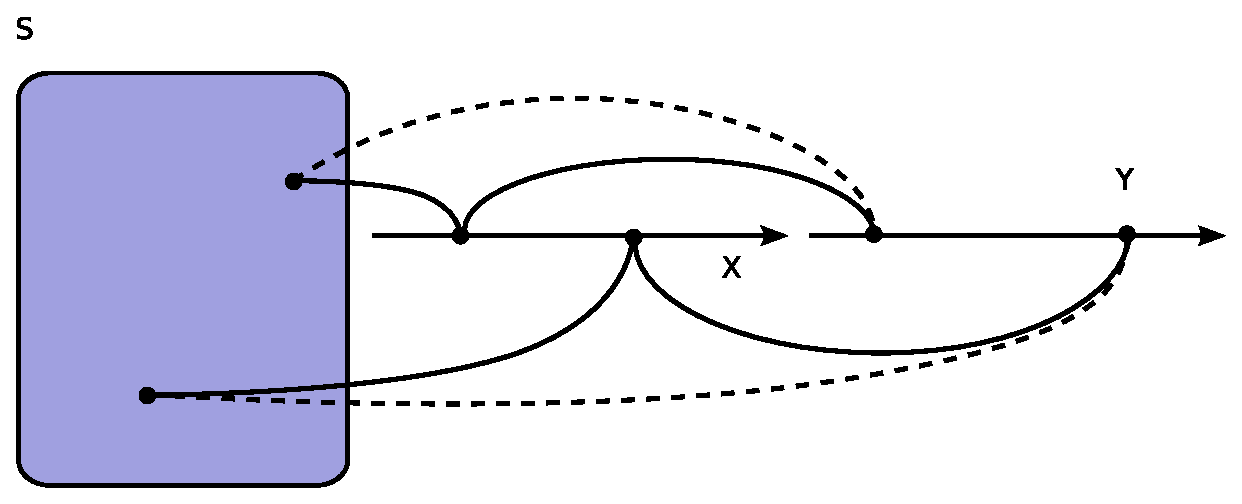
\includegraphics[width=9.26cm]{Figures/9Chapter/fcn-cnt}
\end{psfrags}
\caption{A function of a random variable is a random variable itself.
In this figure, $Y$ is obtained by applying function $g(\cdot)$ to the value of continuous random variable $X$.}
\label{figure:FunctionContinuousRV}
\end{center}
\end{figure}

Let $X$ be a continuous random variable, and let $g: \RealNumbers \mapsto \RealNumbers$ be an admissible function.
Variable $Y = g(X)$, defined pointwise, is itself random.
The probability that $Y$ falls in a specific set $S$ depends on both the function $g(\cdot)$ and the PDF of $X$,
\begin{equation*}
\Pr (Y \in S) = \Pr (g(X) \in S) 
= \Pr \left( X \in g^{-1}(S) \right)
= \int_{g^{-1} (S)} f_X (\xi) d\xi .
\end{equation*}
In particular, we can derive the CDF of $Y$ using the formula
\begin{equation} \label{equation:DerivedCDF}
F_Y(y) = \Pr (g(X) \leq y)
= \int_{ \{ \xi \in X(\Omega) | g(\xi) \leq y \} } f_X(\xi) d\xi .
\end{equation}

\begin{example} \label{example:RayleighExponentialRV}
Let $X$ be a Rayleigh  random variable with parameter $\sigma^2  = 1$, and define $Y = X^2$.
We wish to find the distribution of $Y$.
From \eqref{equation:DerivedCDF}, we can compute the CDF of $Y$.
For $y > 0$, we get
\begin{equation*}
\begin{split}
F_Y(y) &= \Pr (Y \leq y) = \Pr \left( X^2 \leq y \right) \\
&= \Pr (- \sqrt{y} \leq X \leq \sqrt{y})
= \int_0^{\sqrt{y}} \xi e^{- \frac{\xi^2}{2}} d\xi \\
&= \int_0^{y} \frac{1}{2} e^{- \frac{\zeta}{2}} d\zeta
= 1 - e^{-\frac{y}{2}} .
\end{split}
\end{equation*}
Above, we have used the fact that $X \geq 0$ in finding the boundaries of integration, and we made the change of variables $\zeta = \xi^2$ in computing the integral.
We recognize $F_Y(\cdot)$ as the CDF of an exponential random variable.
This shows that the square of a Rayleigh random variable possesses an exponential distribution.
\end{example}

In general, the fact that $X$ is a continuous random variable does not provide much information about the properties of $Y = g(X)$.
For instance, $Y$ could be a continuous random variable, a discrete random variable or neither.
To gain a better understanding of derived distributions, we begin our exposition of functions of continuous random variables by exploring specific cases.


\section{Monotone Functions}

A \emph{monotonic function} is a function that preserves a given order. \index{Monotonic function}
For instance, $g(\cdot)$ is monotone increasing if, for all $x_1$ and $x_2$ such that $x_1 \leq x_2$, we have $g(x_1) \leq g(x_2)$.
Likewise, a function $g(\cdot)$ is termed monotone decreasing provided that $g(x_1) \geq g(x_2)$ whenever $x_1 \leq x_2$.
If the inequalities above are replaced by strict inequalities ($<$ and $>$), then the corresponding functions are said to be \emph{strictly monotonic}. \index{Strictly monotonic function}
Monotonic functions of random variable are straightforward to handle because they allow a simple characterization of derived CDFs.
For non-decreasing function $g(\cdot)$ of continuous random variable $X$, we have
\begin{equation} \label{equation:MonotoneIncreasingCDF}
\begin{split}
F_Y(y) &= \Pr ( Y \leq y) = \Pr ( g(X) \leq y) \\
&= \Pr ( g(X) \in (- \infty, y])
= \Pr ( X \in g^{-1} ( (- \infty, y] ) ) \\
&= \Pr \left( X \leq \sup \left\{ g^{-1} ( (- \infty, y] ) \right\} \right)
= F_X \left( \sup \left\{ g^{-1} ( (- \infty, y] ) \right\} \right) .
\end{split}
\end{equation}
The supremum comes from the fact that multiple values of $x$ may lead to a same value of $y$; that is, the preimage $g^{-1}(y) = \{ x | g(x) = y \}$ may contain several elements.
Furthermore, $g(\cdot)$ may be discontinuous and $g^{-1} (y)$ may not contain any values.
These scenarios all need to be accounted for in our expression, and this is accomplished by selecting the largest value in the set $g^{-1} ( (- \infty, y] )$.

\begin{figure}[ht]
\begin{center}
\begin{psfrags}
\psfrag{x}[c]{$g^{-1} (y) = \{ x | g(x) = y \}$}
\psfrag{y}[c]{$y$}
\psfrag{X}[c]{$X$}
\psfrag{Y}[c]{$Y$}
\includegraphics[width=6.5cm]{Figures/9Chapter/MonotoneIncreasing}
\end{psfrags}
\caption{In this figure, $Y$ is obtained by passing random variable $X$ through a function $g(\cdot)$.
The preimage of point $y$ contains several elements, as seen above.}
\end{center}
\end{figure}

\begin{figure}[ht]
\begin{center}
\begin{psfrags}
\psfrag{x}[c]{$g^{-1} ((-\infty, y])$}
\psfrag{y}[c]{$y$}
\psfrag{X}[c]{$X$}
\psfrag{Y}[c]{$Y$}
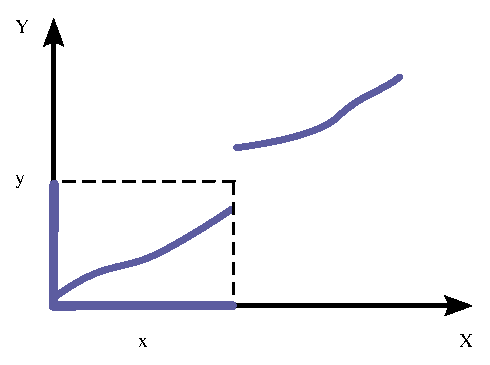
\includegraphics[width=6.5cm]{Figures/9Chapter/Discontinuous}
\end{psfrags}
\caption{If $g(\cdot)$ is discontinuous then $g^{-1} (y)$ may be empty, whereas $g^{-1} ((-\infty, y])$ is typically a well-defined interval.
It is therefore advisable to define $F_Y (y)$ in terms of $g^{-1} ((-\infty, y])$.}
\end{center}
\end{figure}

\begin{example}
Let $X$ be a continuous random variable uniformly distributed over interval $[0, 1]$.
We wish to characterize the derived distribution of $Y = 2X$.
This can be accomplished as follows.
For $y \in [0, 2]$, we get
\begin{equation*}
\begin{split}
F_Y(y) &= \Pr (Y \leq y) = \Pr \left( X \leq \frac{y}{2} \right) \\
&= \int_0^{\frac{y}{2}} dx = \frac{y}{2} .
\end{split}
\end{equation*}
In particular, $Y$ is a uniform random variable with support $[0, 2]$.
By taking derivatives, we obtain the PDF of $Y$ as
\begin{equation*}
f_Y(y) = \begin{cases} \frac{1}{2}, & y \in [0, 2] \\
0, & \text{otherwise}. \end{cases}
\end{equation*}
More generally, an affine function of a uniform random variable is also a uniform random variable.
\end{example}

The same methodology applies to non-increasing functions.
Suppose that $g(\cdot)$ is monotone decreasing, and let $Y = g(X)$ be a function of continuous random variable $X$.
The CDF of $Y$ is then equal to
\begin{equation} \label{equation:MonotoneDecreasingCDF}
\begin{split}
F_Y(y) &= \Pr (Y \leq y) = \Pr \left( X \in g^{-1} ((-\infty, y]) \right) \\
&= \Pr \left( X \geq \inf \left\{ g^{-1} ((-\infty, y]) \right\} \right) \\
&= 1 - F_X \left( \inf \left\{ g^{-1} ((-\infty, y] ) \right\} \right) .
\end{split}
\end{equation}
This formula is similar to the previous case in that the infimum accounts for the fact that the preimage $g^{-1}(y) = \{ x | g(x) = y \}$ may contain numerous elements or no elements at all.


\section{Differentiable Functions}

To further our understanding of derived distributions, we next consider the situation where $g(\cdot)$ is a differentiable and strictly increasing function.
Note that, with these two properties, $g(\cdot)$ becomes an invertible function.
It is therefore possible to write $x = g^{-1} (y)$ unambiguous, as the value of $x$ is unique.
In such a case, the CDF of $Y = g(X)$ becomes
\begin{equation*}
F_Y(y) = \Pr \left( X \leq g^{-1}(y) \right)
= F_X \left( g^{-1} (y) \right) .
\end{equation*}
Differentiating this equation with respect to $y$, we obtain the PDF of $Y$
\begin{equation*}
\begin{split}
f_Y (y) &= \frac{d}{dy} F_Y(y)
= \frac{d}{dy} F_X \left( g^{-1} (y) \right) \\
&= f_X \left( g^{-1} (y) \right) \frac{d}{dy} g^{-1} (y)
= f_X \left( g^{-1} (y) \right) \frac{dx}{dy} .
\end{split}
\end{equation*}
With the simple substitution $x = g^{-1} (y)$, we get
\begin{equation*}
f_Y (y) = f_X (x) \frac{dx}{dy}
= \frac{f_X (x)}{\frac{dg}{dx}(x)} .
\end{equation*}
Note that $\frac{dg}{dx} (x)$ is non-zero because $g(\cdot)$ is a strictly increasing function.
From this analysis, we gather that $Y=g(X)$ is a continuous random variable.
In addition, when $g(\cdot)$ is differentiable and strictly increasing, we can express the PDF of $Y = g(X)$ in terms of the PDF of $X$ and the derivative of $g(\cdot)$, as seen above.

\begin{figure}[ht]
\begin{center}
\begin{psfrags}
\psfrag{x1}[c]{\footnotesize $g^{-1} ((y_1, y_1 + \delta))$}
\psfrag{x2}[c]{\footnotesize $g^{-1} ((y_2, y_2 + \delta))$}
\psfrag{y1}[r]{\footnotesize $(y_1, y_1 + \delta)$}
\psfrag{y2}[r]{\footnotesize $(y_2, y_2 + \delta)$}
\psfrag{X}[c]{$X$}
\psfrag{Y}[c]{$Y$}
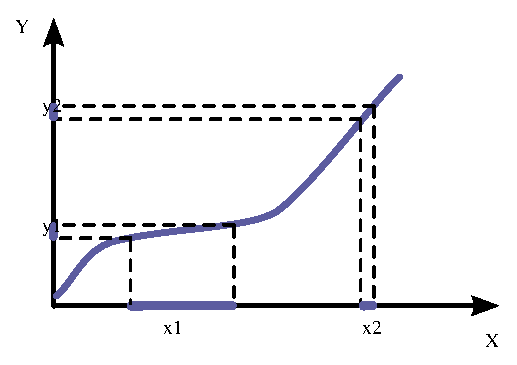
\includegraphics[width=6.5cm]{Figures/9Chapter/Differentiable}
\end{psfrags}
\caption{This figure provides a graphical interpretation of why the derivative of $g(\cdot)$ plays an important role in determining the value of the derived PDF $f_Y(\cdot)$.
For an interval of width $\delta$ on the $y$-axis, the size of the corresponding interval on the $x$-axis depends heavily on the derivative of $g(\cdot)$.
A small slope leads to a wide interval, whereas a steep slope produces a narrow interval on the $x$-axis.}
\label{figure:DifferentiablePDF}
\end{center}
\end{figure}

Likewise, suppose that $g(\cdot)$ is differentiable and strictly decreasing.
We can write the CDF of random variable $Y = g(X)$ as follows,
\begin{equation*}
F_Y(y) = \Pr (g(X) \leq y)
= \Pr \left( X \geq g^{-1}(y) \right)
= 1 - F_X \left( g^{-1} (y) \right) ;
\end{equation*}
and its PDF is given by
\begin{equation*}
\begin{split}
f_Y (y) &= \frac{d}{dy} \left( 1 - F_X \left( g^{-1} (y) \right) \right)
%= - f_X \left( g^{-1} (y) \right) \frac{dx}{dy}
= \frac{f_X (x)}{- \frac{dg}{dx}(x)} ,
\end{split}
\end{equation*}
where again $x = g^{-1} (y)$.
As before, we find that $Y = g(X)$ is a continuous random variable and the PDF of $Y$ can be expressed in therms of $f_X( \cdot)$ and the derivative of $g(\cdot)$.
Combining these two results, we observe that if $g(\cdot)$ is differentiable and strictly monotone, the PDF of $Y$ becomes
\begin{equation} \label{equation:MonotoneFunctionPDF}
f_Y (y) = f_X \left( g^{-1} (y) \right) \left| \frac{dx}{dy} \right|
= \frac{f_X (x)}{\left| \frac{dg}{dx}(x) \right|}
\end{equation}
where $x = g^{-1}(y)$.
The role of $\frac{dg}{dx} (\cdot)$ in finding the derived PDF $f_Y(\cdot)$ is illustrated in Figure~\ref{figure:DifferentiablePDF}.

\begin{example}
Suppose that $X$ is a Gaussian random variable with PDF
\begin{equation*}
f_X(x) = \frac{1}{\sqrt{2 \pi}} e^{- \frac{x^2}{2}} .
\end{equation*}
We wish to find the PDF of random variable $Y$ where $Y = a X + b$ and $a \neq 0$.

In this example, we have $g(x) = ax + b$ and $g(\cdot)$ is immediately recognized as a strictly monotonic function.
The inverse of function of $g(\cdot)$ is equal to
\begin{equation*}
x = g^{-1} (y) = \frac{y - b}{a} ,
\end{equation*}
and the desired derivative is given by
\begin{equation*}
\frac{dx}{dy} = \frac{1}{\frac{dg}{dx} (x)} = \frac{1}{a} .
\end{equation*}
The PDF of $Y$ can be computed using \eqref{equation:MonotoneFunctionPDF}, and is found to be
\begin{equation*}
f_Y(y) = f_X \left( g^{-1} (y) \right) \left| \frac{dx}{dy} \right|
= \frac{1}{\sqrt{2 \pi} |a|} e^{- \frac{(y-b)^2}{2 a^2} } ,
\end{equation*}
which is itself a Gaussian distribution.
Using a similar progression, we can show that an affine function of a Gaussian random variable is always a Gaussian random variable.
\end{example}

\begin{example}
Suppose $X$ is a Rayleigh random variable with parameter $\sigma^2 = 1$, and let $Y = X^2$.
We wish to derive the distribution of random variable $Y$ using the PDF of $X$.

Recall that the distribution of Rayleigh random variable $X$ is given by
\begin{equation*}
f_X (x) = x e^{- \frac{x^2}{2} } \quad x \geq 0.
\end{equation*}
Since $Y$ is the square of $X$, we have $g(x) = x^2$.
Note that $X$ is a non-negative random variable and $g(x) = x^2$ is strictly monotonic over $[0, \infty)$.
The PDF of $Y$ is therefore found to be
\begin{equation*}
f_Y(y) = \frac{f_X (x)}{\left| \frac{dg}{dx}(x)\right|}
= \frac{f_X \left( \sqrt{y} \right)}{\left| \frac{dg}{dx} \left( \sqrt{y} \right) \right|}
= \frac{\sqrt{y}}{2 \sqrt{y}} e^{- \frac{y}{2} }
= \frac{1}{2} e^{- \frac{y}{2} } ,
\end{equation*}
where $y \geq 0$.
Thus, random variable $Y$ possesses an exponential distribution with parameter $1 / 2$.
It may be instructive to compare this derivation with the steps outlined in Example~\ref{example:RayleighExponentialRV}.
\end{example}

Finally, suppose that $g(\cdot)$ is a differentiable function with a finite number of local extrema.
Then, $g(\cdot)$ is piecewise monotonic and we can write the PDF of $Y= g(X)$ as
\begin{equation} \label{equation:FunctionPDF}
f_Y (y) = \sum_{ \{ x \in X(\Omega) | g(x) = y \} }
\frac{f_X (x)}{\left| \frac{dg}{dx}(x) \right|}
\end{equation}
for (almost) all values of $y \in \RealNumbers$.
That is, $f_Y (y)$ is obtained by first identifying the values of $x$ for which $g(x) = y$.
The PDF of $Y$ is then computed explicitly by finding the local contribution of each of these values to $f_Y(y)$ using the methodology developed above.
This is accomplished by applying \eqref{equation:MonotoneFunctionPDF} repetitively to every value of $x$ for which $g(x) = y$.
% This is illustrated in Figure.
It is certainly useful to compare \eqref{equation:FunctionPDF} to its discrete equivalent \eqref{equation:DefinitionFunctionPMF}, which is easier to understand and visualize.

\begin{figure}[ht]
\begin{center}
\begin{psfrags}
\psfrag{y}[c]{$y$}
\psfrag{x1}[c]{$x_1$}
\psfrag{x2}[c]{$x_2$}
\psfrag{x3}[c]{$x_3$}
\psfrag{x4}[c]{$x_4$}
\psfrag{x5}[c]{$x_5$}
\psfrag{X}[c]{$X$}
\psfrag{Y}[c]{$Y$}
\includegraphics[width=6.5cm]{Figures/9Chapter/DerivedPDF}
\end{psfrags}
\caption{The PDF of $Y = g(X)$ when $X$ is a continuous random variable and $g(\cdot)$ is differentiable with a finite number of local extrema is obtained by first identifying all the values of $x$ for which $g(x) = y$, and then calculating the contribution of each of these values to $f_Y(y)$ using \eqref{equation:MonotoneFunctionPDF}.
The end result leads to \eqref{equation:FunctionPDF}.}
\end{center}
\end{figure}

\begin{example}
Suppose $X$ is a continuous random variable uniformly distributed over $[0, 2 \pi)$.
Let $Y = \cos (X)$, the random sampling of a sinusoidal waveform.
We wish to find the PDF of $Y$.

For $y \in (-1, 1)$, the preimage $g^{-1} (y)$ contains two values in $[0, 2\pi)$, namely $\arccos (y)$ and $(2 \pi - \arccos (y))$.
Recall that the derivative of $\cos(x)$ is given by
\begin{equation*}
\frac{d}{dx} \cos (x) = - \sin (x) .
\end{equation*}
Collecting these results, we can write the PDF of $Y$ as
\begin{equation*}
\begin{split}
f_Y (y) &= \frac{f_X( \arccos (y) )}{ \left| - \sin (\arccos (y)) \right|}
+ \frac{f_X( 2 \pi - \arccos (y) )}{ \left| - \sin (2\pi - \arccos (y)) \right| } \\
&= \frac{1}{2 \pi \sqrt{1 - y^2} } + \frac{1}{ 2 \pi \sqrt{ 1 - y^2} }
= \frac{1}{\pi \sqrt{1 - y^2} } ,
\end{split}
\end{equation*}
where $-1 < y < 1$.
The CDF of $Y$ can be obtained by integrating $f_Y (y)$.
Not surprisingly, solving this integral involves a trigonometric substitution.
\end{example}


\section{Generating Random Variables}

In many engineering projects, computer simulations are employed as a first step in validating concepts or comparing various design candidates.
Many such tasks involve the generation of random variables.
In this section, we explore a method to generate arbitrary random variables based on a routine that outputs a random value uniformly distributed between zero and one.

\subsection{Continuous Random Variables}

First, we consider a scenario where the simulation task requires the generation of a continuous random variable.
We begin our exposition with a simple observation.
Let $X$ be a continuous random variable with PDF $f_X (\cdot)$.
Consider the random variable $Y = F_X(X)$.
Since $F_X (\cdot)$ is differentiable and strictly increasing over the support of $X$, we get
\begin{equation*}
f_Y (y) = \frac{f_X (x)}{\left| \frac{d F_X}{dx} (x) \right|}
= \frac{f_X (x)}{| f_X (x) |} = 1
\end{equation*}
where $y \in (0, 1)$ and $x = F_X^{-1} (y)$.
The PDF of $Y$ is zero outside of this interval because $0 \leq F_X (x) \leq 1$.
Thus, using an arbitrary continuous random variable $X$, we can generate a uniform random variable $Y$ with PDF
\begin{equation*}
f_Y(y) = \begin{cases} 1 & y \in (0,1) \\
0 & \text{otherwise} . \end{cases}
\end{equation*}

This observation provides valuable insight about our original goal.
Suppose that $Y$ is a continuous random variable uniformly distributed over $[0,1]$.
We wish to generate continuous random variable with CDF $F_X(\cdot)$.
First, we note that, when $F_X (\cdot)$ is invertible, we have
\begin{equation*}
F_X^{-1} \left( F_X (X) \right) = X .
\end{equation*}
Thus, applying $F_X^{-1} (\cdot)$ to uniform random variable $Y$ should lead to the desired result.
Define $V = F_X^{-1} (Y)$, and consider the PDF of $V$.
Using our knowledge of derived distributions, we get
\begin{equation*}
\begin{split}
f_V (v) = \frac{ f_Y (y) }{ \left| \frac{d F_X^{-1}}{dy} (y) \right| }
= f_Y (y) \frac{d F_X}{dv} (v) = f_X (v)
\end{split}
\end{equation*}
where $y = F_X (v)$.
Note that $f_Y (y) = 1$ for any $y \in [0,1]$ because $Y$ is uniform over the unit interval.
We stress that this technique can be utilized to generate any random variable with PDF $f_X (\cdot)$ from a computer routine that outputs a random value uniformly distributed between zero and one.
In other words, to create a continuous random variable $X$ with CDF $F_X (\cdot)$, one can apply the function $F_X^{-1} (\cdot)$ to a random variable $Y$ that is uniformly distributed over $[0,1]$.

\begin{example}
Suppose that $Y$ is a continuous random variable uniformly distributed over $[0,1]$.
We wish to create an exponential random variable $X$ with parameter $\lambda$ by taking a function of $Y$.

Random variable $X$ is nonnegative, and its CDF is given by $F_X(x) = 1 - e^{- \lambda x}$ for $x \geq 0$.
The inverse of $F_X (\cdot)$ is given by
\begin{equation*}
F_X^{-1} (y) = - \frac{1}{\lambda} \log (1 - y) .
\end{equation*}
We can therefore generate the desired random variable $X$ with
\begin{equation*}
X = - \frac{1}{\lambda} \log (1 - Y) .
\end{equation*}
Indeed, for $x \geq 0$, we obtain
\begin{equation*}
f_X (x) = \frac{ f_Y (y) }{ \frac{1}{\lambda (1 - y)} }
= \lambda e^{- \lambda x}
\end{equation*}
where we have implicitly defined $y = 1 - e^{- \lambda x}$.
This is the desired distribution.
\end{example}


\subsection{Discrete Random Variables}

It is equally straightforward to generate a discrete random variable from a continuous random variable that is uniformly distributed between zero and one.
Let $p_X(\cdot)$ be a PMF, and denote its support by $\{ x_1, x_2, \ldots \}$ where $x_i < x_j$ whenever $i < j$.
We know that the corresponding CDF is given by
\begin{equation*}
F_X(x) = \sum_{x_i \leq x} p_X (x_i) .
\end{equation*}
We can generate a random variable $X$ with PMF $p_X(\cdot)$ with the following function,
\begin{equation*}
g(y) = \begin{cases} x_i, & \text{if } F_X(x_{i-1}) < y \leq F_X (x_i) \\
0, & \text{otherwise}. \end{cases}
\end{equation*}
Note that we have used the convention $x_0 = 0$ to simplify the definition of $g(\cdot)$.
Taking $X = g(Y)$, we get
\begin{equation*}
\begin{split}
\Pr (X = x_i) &= \Pr ( F_X(x_{i-1}) < Y \leq F_X (x_i) ) \\
&= F_X (x_i) - F_X (x_{i-1}) = p_X (x_i) .
\end{split}
\end{equation*}
Of course, implementing a discrete random variable through a case statement may lead to an excessively slow routine.
For many discrete random variables, there are much more efficient ways to generate the desired output.


\section{Discrete Approximations*}

Traditionally, the study of complex systems has relied on empirical observations and abstract mathematical models that are amenable to analysis.
The hope is that such an approach will lead to accurate predictions about the behavior of the underlying system, under various parameters and initial conditions.
While this approach has had and continues to have many successes, the immense capabilities of contemporary computer servers has enabled the complementary means of numerical methods.
Computer simulations now play a key role in the analysis of many complex systems, permitting the study of entities and mechanisms that are otherwise not amenable to analysis.
Monte Carlo techniques and other numerical simulations are used extensively in almost all areas of engineering and physical sciences.
Moreover, algorithms that make random decisions during their execution, termed \emph{randomized algorithms}, are widespread in numerical simulations. \index{Randomized algorithms}

When using computers to study continuous mathematics, discretization techniques must be applied.
The study of efficient discrete algorithms that provide accurate approximations to continuous problems is known as \emph{numerical analysis}.
Problems in one dimension can usually be handled very precisely through finite precision arithmetic, as the number of bits used to represent numbers in modern computers is vast.
For example, computer routines are used extensively to simulate continuous random variables.
In higher dimensions, care must be taken to discretize volumes and approximate local interactions.
Potential discretization techniques include finite element methods, finite differences and high-resolution schemes.


\section*{Further Reading}

\begin{small}
\begin{enumerate}
\item Ross, S., \emph{A First Course in Probability}, 7th edition, Pearson Prentice Hall, 2006: Section~5.7.
\item Bertsekas, D.P., and Tsitsiklis, J.N., \emph{Introduction to Probability}, Athena Scientific, 2002: Section~3.6.
\item Mitzenmacher, M., and Upfal, E., \emph{Probability and Computing: Randomized Algorithms and Probabilistic Analysis}, Cambridge, 2005: Chapters~1~\&~10.
\end{enumerate}
\end{small}

